\newpage
\section{Train Results}
\label{sec:trainresults}

In this section we present the results obtained by our systems. In particular, Section 4 summarizes the system's performance with different configurations on the training dataset. 

We evaluated different configurations of our search engine by integrating the components described in Section 2 and tuning their parameters for optimal performance. Table ~\ref{tab:evaluation_results} reports the MAP and nDCG scores for each method, based on test data and relevance judgments of the 2023/01 dataset.

\begin{table}[ht]
\centering
\caption{Evaluation results on MAP and NDCG for different methods}
\label{evaluations_results}
\begin{tabular}{|l|c|c|}
\hline
\rowcolor{gray!20}
\textbf{Method} & \textbf{MAP} & \textbf{NDCG} \\
\hline
\multicolumn{3}{|l|}{\footnotesize\textit{Tokenizers}} \\
Whitespace                     & 0.1855 & 0.2847 \\
Letter                         & \textbf{0.2002} & \textbf{0.3061} \\
Standard                       & 0.2002 & 0.3059 \\
NLP                            & 0.1892 & 0.2906 \\
\hline
\multicolumn{3}{|l|}{\footnotesize\textit{Stemmers}} \\
FrenchLight                    & 0.1722 & 0.2745 \\
FrenchMinimal                  & 0.1798 & 0.2832 \\
Snowball                       & 0.1848 & 0.2903 \\
\hline
\multicolumn{3}{|l|}{\footnotesize\textit{Analyzer methods}} \\
Expansion               & 0.2000 & 0.3058 \\
Position                & 0.2002 & 0.3061 \\
Double                  & 0.2003 & 0.3063 \\
PositionOpnNLP          & \textbf{0.2011} & \textbf{0.3069} \\
\hline
\multicolumn{3}{|l|}{\footnotesize\textit{Other Methods}} \\
Dictionary                                          & 0.2014 & 0.3072 \\
Synonyms                                            & 0.1979 & 0.3034 \\
Fuzzy                                               & 0.2135 & 0.3230 \\
Phrase                                              & 0.2243 & 0.3270 \\
PRF                                                 & 0.1768 & 0.2905 \\
Word2vec                                            & 0.1689 & 0.2814 \\
N-grams                                             & 0.2002 & 0.3061 \\
Heuristic                                           & 0.1361 & 0.2237 \\
Start                                               & 0.2011 & 0.3069 \\
Highlights                                          & 0.2002 & 0.3062 \\
Phrase + Fuzzy + Start                              & 0.2359 & 0.3422 \\
Phrase + Fuzzy + Start + Highlights                 & 0.2359 & 0.3423 \\
Phrase + Fuzzy + Start + N-grams                    & 0.2359 & 0.3422 \\
Phrase + Fuzzy + Start + dictionary                 & 0.2355 & 0.3420 \\
Phrase + Fuzzy + Start + Highlights + Doubles       & 0.2359 & 0.3423 \\
Phrase + Fuzzy + Start + Highlights + Reranker      & 0.2585 & 0.3600 \\
Phrase + Fuzzy + Start + Highlights + Doubles + Reranker      & \textbf{0.2585} & \textbf{0.3601} \\
\hline
\end{tabular}
\begin{tablenotes}
\footnotesize
\item Bold numbers indicate the best-performing configuration. All methods in each section use the best parameter values from the preceding sections.
\end{tablenotes}
\end{table}


\textbf{Tokenizers}:

Among the tokenizers, the Letter Tokenizer achieved the best results, slightly outperforming the Standard Tokenizer. In contrast, the Whitespace Tokenizer yielded poorer retrieval performance, while the NLP tokenizer was slower and less effective due to its computational overhead.

\vspace{1\baselineskip}
\textbf{Stemmers}:

All stemmers negatively impacted retrieval performance and were therefore excluded from subsequent configurations.

\vspace{1\baselineskip}
\textbf{Analyzer Methods}:

We extended our analysis using the Letter Tokenizer and stopword filtering as a baseline, applying expansion, position-based weighting, and OpenNLP-based position tagging. Among these, only OpenNLP position tagging provided a performance improvement.

\vspace{1\baselineskip}
\textbf{Other Methods}:

To enable a systematic and manageable evaluation, each method was primarily tested in isolation under the simplifying assumption that components do not interact. This approach allowed us to isolate and measure the individual contribution of each feature. Features that did not yield improvements were excluded from subsequent configurations.

Neutral or beneficial features were tested in combination to assess potential performance gains. In the case of the dictionary, although it showed improvement in isolation, its integration with other configurations led to a decrease in performance.

The combination of Phrase, Fuzzy, Start, Highlights, and Reranker yielded the best results, and its features were adopted in the following evaluation stages.


\section{Test Results}
\label{sec:testresults}

In this Section we will show and analyze the results obtained by our system.
In particular, Section~\ref{subsec:train-res} will be about the results of all the runs produced by our system on the training collection during its development, while Section~\ref{subsec:test-res} will consist of a statistical analysis of the runs submitted to \ac{CLEF} on the test collections.

\subsubsection{explanations }
\label{subsubsec:heldout-res}


\newcolumntype{C}{>{\centering\arraybackslash}X}

\begin{table}[tbp]
\centering
\caption{\ac{nDCG} and \ac{MAP} values - Baseline: Phrase + Fuzzy + Start + Highlights}
\label{tab:heldout-map-ndcg-table-transposed}
\begin{tabularx}{\textwidth}{|l|C|C|C|C|}
\toprule
\textbf{Date} & \textbf{Baseline} & \textbf{Baseline + Reranker\_50} & \textbf{Baseline + Correction + Reranker\_50}  \\
\midrule
2023/3 & 0.2394 - 0.3449 & 0.2706 - 0.3703 & 0.2707 - 0.3704\\
2023/4 & 0.2566 - 0.3682 & 0.2804 - 0.3865 & 0. - 0. \\
2023/5 & 0.2515 - 0.3603 & 0.2802 - 0.3830 & 0.2796 - 0.3823 \\
2023/6 & 0.2685 - 0.3756 & 0.2973 - 0.3985 & 0.2970 - 0.3982 \\
2023/7 & 0.2475 - 0.3539 & 0.2715 - 0.3736 & 0.2706 - 0.3725 \\
2023/8 & 0.2208 - 0.3095 & 0.2375 - 0.3209 & 0.2355 - 0.3207 \\
\bottomrule
\end{tabularx}
\end{table}


\begin{table}[tbp]
\footnotesize
\centering
\caption{\ac{nDCG} and \ac{MAP} values - Baseline: Phrase + Fuzzy + Start + Highlights}
\label{tab:heldout-map-ndcg-table-transposed}
\begin{tabularx}{\textwidth}{@{} l *{3}{>{\centering\arraybackslash}X} @{}}
\toprule
\textbf{Date} & \textbf{Baseline} & \textbf{Baseline + Reranker\_50} & \textbf{Baseline + Correction + Reranker\_50}  \\
\midrule
2023/3 & 0.2394 - 0.3449 & 0.2706 - 0.3703 & 0.2707 - 0.3704 \\
2023/4 & 0.2566 - 0.3682 & 0.2804 - 0.3865 & 0. - 0. \\
2023/5 & 0.2515 - 0.3603 & 0.2802 - 0.3830 & 0.2796 - 0.3823 \\
2023/6 & 0.2685 - 0.3756 & 0.2973 - 0.3985 & 0.2970 - 0.3982 \\
2023/7 & 0.2475 - 0.3539 & 0.2715 - 0.3736 & 0.2706 - 0.3725 \\
2023/8 & 0.2208 - 0.3095 & 0.2375 - 0.3209 & 0.2355 - 0.3207 \\
\bottomrule
\end{tabularx}
\end{table}

\vspace{-1em} % riduce spazio tra le due tabelle

\begin{table}[tbp]
\footnotesize
\centering
\caption{ANOVA2 on heldout collection}
\label{tab:heldout-anova2}


\begin{tabularx}{\textwidth}{@{} l *{5}{>{\centering\arraybackslash}X} l *{5}{>{\centering\arraybackslash}X} @{}}
\toprule
\multicolumn{6}{c}{\textbf{\ac{nDCG 2023/03}}} & \multicolumn{5}{c}{\textbf{\ac{AP 2023/03}}} \\
\midrule
\textbf{Source} & \textbf{SS} & \textbf{df} & \textbf{MS} & \textbf{F} & \textbf{Prob$>$F} & \textbf{SS} & \textbf{df} & \textbf{MS} & \textbf{F} & \textbf{Prob$>$F} \\
\midrule
Systems & 2.2037    & 2     & 1.1018 & 99.2415  & 1.11e-16 & 3.3111    & 2     & 1.6556 & 104.3786 & 1.11e-16 \\
Topics  & 1516.7022 & 5091  & 0.2979 & 26.8332  & 1.11e-16 & 1656.7083 & 5091  & 0.3254 & 20.5169  & 1.11e-16 \\
Error   & 113.0466  & 10182 & 0.0111 & -        & -        & 161.4973  & 10182 & 0.0159 & -        & -        \\
Total   & 1631.9525 & 15275 & -      & -        & -        & 1821.5167 & 15275 & -      & -        & -        \\
\bottomrule
\end{tabularx}

\vspace{1em}

\begin{tabularx}{\textwidth}{@{} l *{5}{>{\centering\arraybackslash}X} @{\hspace{1em}} l *{5}{>{\centering\arraybackslash}X} @{}}
\toprule
\multicolumn{6}{c}{\textbf{\ac{nDCG 2023/04}}} & \multicolumn{5}{c}{\textbf{\ac{AP 2023/04}}} \\
\midrule
\textbf{Source} & \textbf{SS} & \textbf{df} & \textbf{MS} & \textbf{F} & \textbf{Prob$>$F} & \textbf{SS} & \textbf{df} & \textbf{MS} & \textbf{F} & \textbf{Prob$>$F} \\
\midrule
Systems & 2.8477    & 2     & 1.4238 & 142.4028 & 1.11e-16  & 4.8140    & 2     & 2.4070 & 167.9370 & 1.11e-16 \\
Topics  & 3833.4804 & 13019 & 0.2945 & 29.4491  & 1.11e-16  & 4280.9664 & 13019 & 0.3288 & 22.9423  & 1.11e-16 \\
Error   & 260.3461  & 26038 & 0.0100 & -        & -         & 373.1943  & 26038 & 0.0143 & -        & -        \\
Total   & 4096.6742 & 39059 & -      & -        & -         & 4658.9747 & 39059 & -      & -        & -        \\
\bottomrule
\end{tabularx}

\begin{tabularx}{\textwidth}{@{} l *{5}{>{\centering\arraybackslash}X} @{\hspace{1em}} l *{5}{>{\centering\arraybackslash}X} @{}}
\toprule
\multicolumn{6}{c}{\textbf{\ac{nDCG 2023/05}}} & \multicolumn{5}{c}{\textbf{\ac{AP 2023/05}}} \\
\midrule
\textbf{Source} & \textbf{SS} & \textbf{df} & \textbf{MS} & \textbf{F} & \textbf{Prob$>$F} & \textbf{SS} & \textbf{df} & \textbf{MS} & \textbf{F} & \textbf{Prob$>$F} \\
\midrule
Systems & 3.5115    & 2     & 1.7557 & 180.8835 & 1.11e-16  & 5.6599    & 2     & 2.8300 & 201.4644 & 1.11e-16 \\
Topics  & 3137.5278 & 10540 & 0.2977 & 30.6681  & 1.11e-16  & 3475.6841 & 10540 & 0.3298 & 23.4756  & 1.11e-16 \\
Error   & 204.6118  & 21080 & 0.0097 & -        & -         & 296.1097  & 21080 & 0.0140 & -        & -        \\
Total   & 3345.6511 & 31622 & -      & -        & -         & 3777.4538 & 31622 & -      & -        & -        \\
\bottomrule
\end{tabularx}

\begin{tabularx}{\textwidth}{@{} l *{5}{>{\centering\arraybackslash}X} @{\hspace{1em}} l *{5}{>{\centering\arraybackslash}X} @{}}
\toprule
\multicolumn{6}{c}{\textbf{\ac{nDCG 2023/06}}} & \multicolumn{5}{c}{\textbf{\ac{AP 2023/06}}} \\
\midrule
\textbf{Source} & \textbf{SS} & \textbf{df} & \textbf{MS} & \textbf{F} & \textbf{Prob$>$F} & \textbf{SS} & \textbf{df} & \textbf{MS} & \textbf{F} & \textbf{Prob$>$F} \\
\midrule
Systems & 2.4794    & 2     & 1.2397 & 100.8968 & 1.11e-16  & 3.9272    & 2     & 1.9636 & 110.6254 & 1.11e-16 \\
Topics  & 2233.7190 & 7203  & 0.3101 & 25.2389  & 1.11e-16  & 2471.6517 & 7203  & 0.3431 & 19.3319  & 1.11e-16 \\
Error   & 177.0063  & 14406 & 0.0123 & -        & -         & 255.7065  & 14406 & 0.0178 & -        & -        \\
Total   & 2413.2047 & 21611 & -      & -        & -         & 2731.2854 & 21611 & -      & -        & -        \\
\bottomrule
\end{tabularx}

\begin{tabularx}{\textwidth}{@{} l *{5}{>{\centering\arraybackslash}X} @{\hspace{1em}} l *{5}{>{\centering\arraybackslash}X} @{}}
\toprule
\multicolumn{6}{c}{\textbf{\ac{nDCG 2023/07}}} & \multicolumn{5}{c}{\textbf{\ac{AP 2023/07}}} \\
\midrule
\textbf{Source} & \textbf{SS} & \textbf{df} & \textbf{MS} & \textbf{F} & \textbf{Prob$>$F} & \textbf{SS} & \textbf{df} & \textbf{MS} & \textbf{F} & \textbf{Prob$>$F} \\
\midrule
Systems & 2.1803    & 2     & 1.0902 & 110.1607 & 1.11e-16  & 3.3034    & 2     & 1.6517 & 115.5261 & 1.11e-16 \\
Topics  & 2652.5206 & 8946  & 0.2965 & 29.9616  & 1.11e-16  & 2857.5674 & 8946  & 0.3194 & 22.3420  & 1.11e-16 \\
Error   & 177.0613  & 17892 & 0.0099 & -        & -         & 255.8024  & 17892 & 0.0143 & -        & -        \\
Total   & 2831.7623 & 26840 & -      & -        & -         & 3116.6731 & 26840 & -      & -        & -        \\
\bottomrule
\end{tabularx}

\begin{tabularx}{\textwidth}{@{} l *{5}{>{\centering\arraybackslash}X} @{\hspace{1em}} l *{5}{>{\centering\arraybackslash}X} @{}}
\toprule
\multicolumn{6}{c}{\textbf{\ac{nDCG 2023/08}}} & \multicolumn{5}{c}{\textbf{\ac{AP 2023/08}}} \\
\midrule
\textbf{Source} & \textbf{SS} & \textbf{df} & \textbf{MS} & \textbf{F} & \textbf{Prob$>$F} & \textbf{SS} & \textbf{df} & \textbf{MS} & \textbf{F} & \textbf{Prob$>$F} \\
\midrule
Systems & 0.9767    & 2     & 0.4884 & 60.6778  & 1.11e-16  & 1.6796    & 2     & 0.8398 & 74.3744  & 1.11e-16 \\
Topics  & 3496.3967 & 11551 & 0.3027 & 37.6084  & 1.11e-16  & 3418.7098 & 11551 & 0.2960 & 26.2108  & 1.11e-16 \\
Error   & 185.9371  & 23102 & 0.0080 & -        & -         & 260.8629  & 23102 & 0.0113 & -        & -        \\
Total   & 3683.3105 & 34655 & -      & -        & -         & 3681.2524 & 34655 & -      & -        & -        \\
\bottomrule
\end{tabularx}

\end{table}


\begin{tabular}{|c|c|c|}
\hline
\textbf{Data} & \textbf{nDCG} & \textbf{AP} \\
\hline
2023/03 & 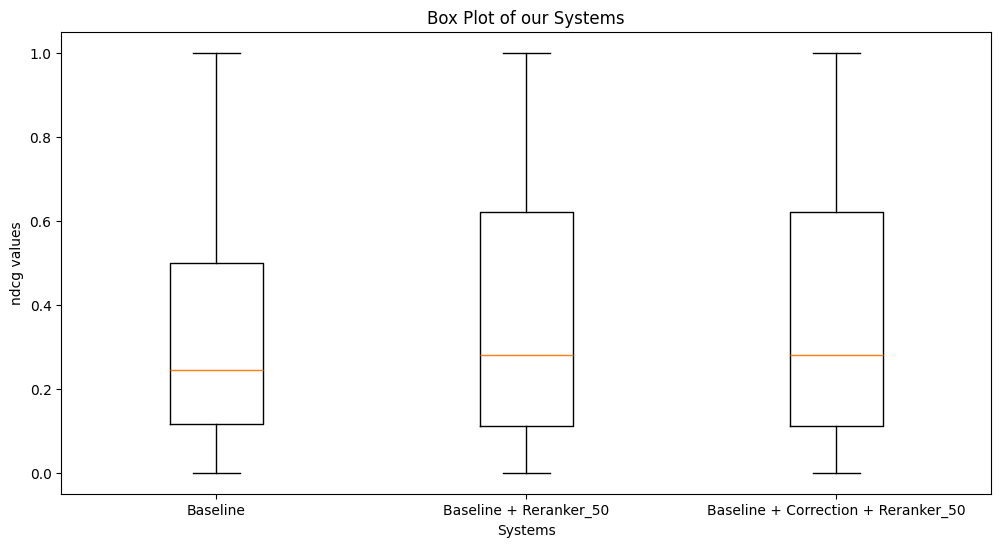
\includegraphics[height=3.5cm]{figure/box_ndcg_3.png} & 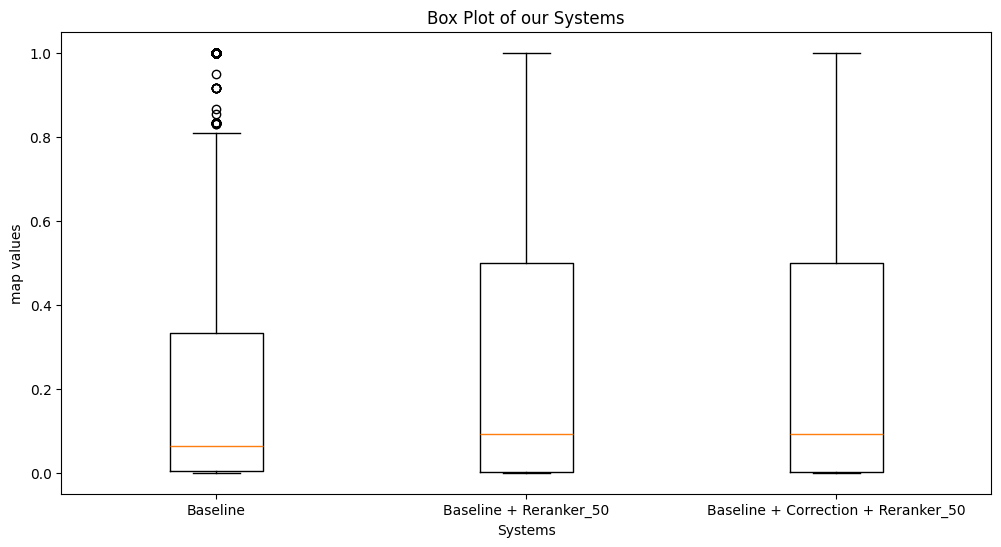
\includegraphics[height=3.5cm]{figure/box_ap_3.png} \\
2023/04 & 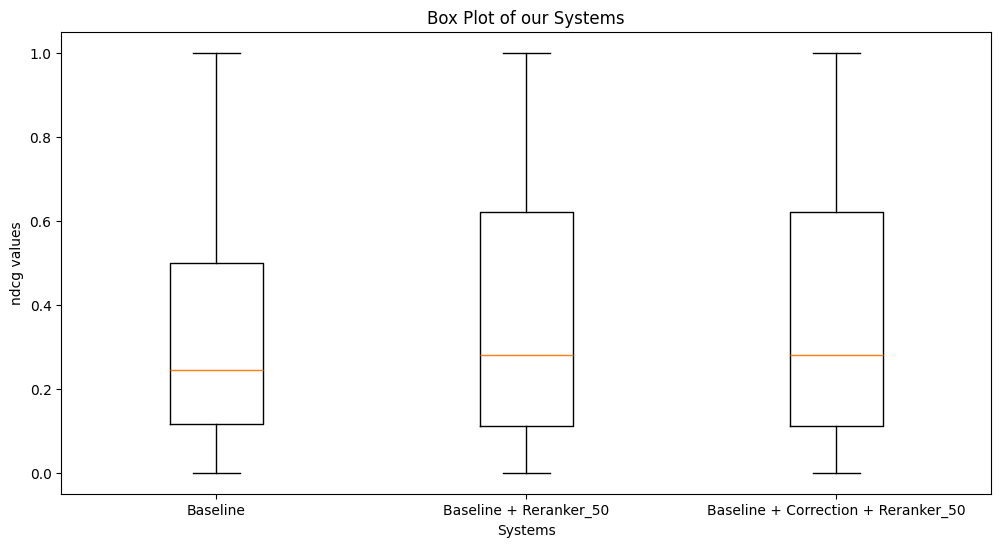
\includegraphics[height=3.5cm]{figure/box_ndcg_3.png} & 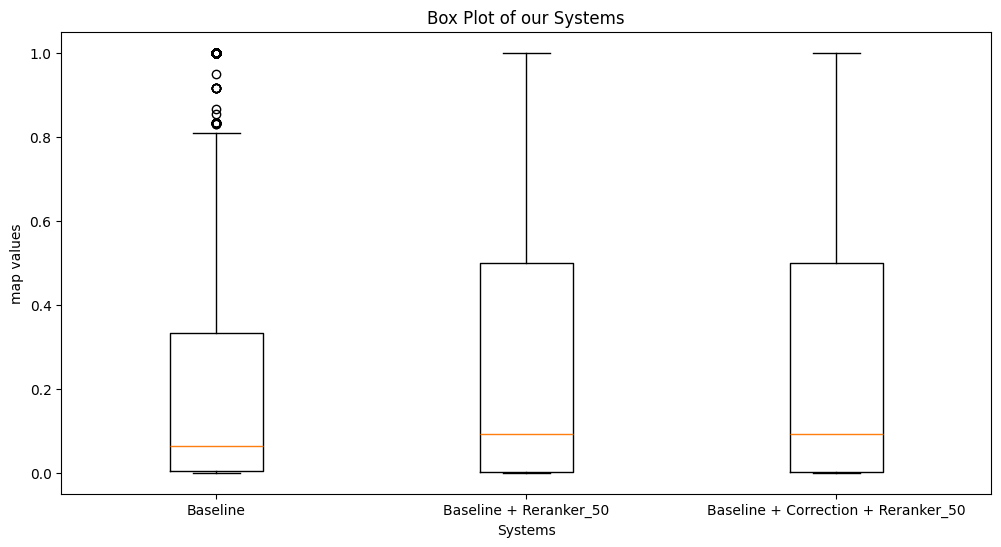
\includegraphics[height=3.5cm]{figure/box_ap_3.png} \\
2023/05 & 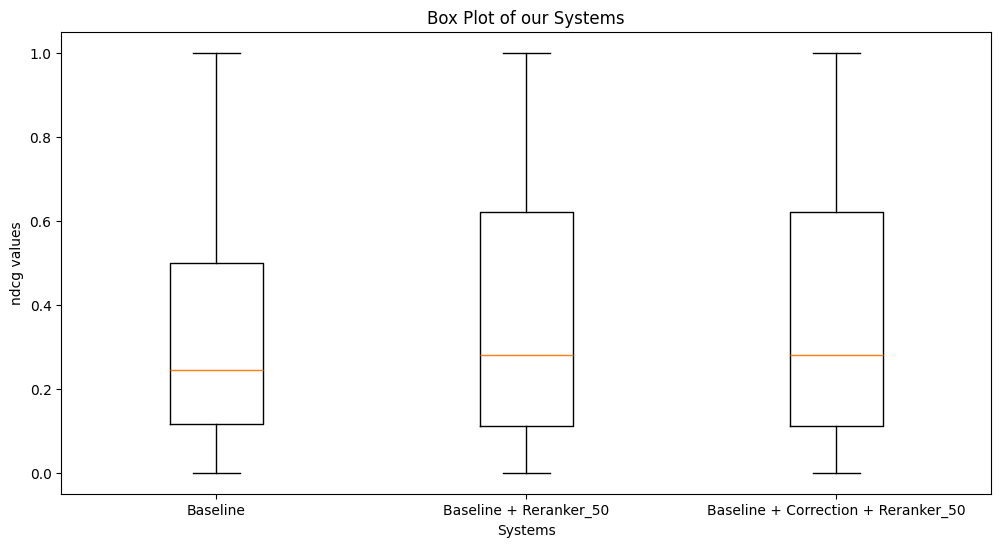
\includegraphics[height=3.5cm]{figure/box_ndcg_3.png} & 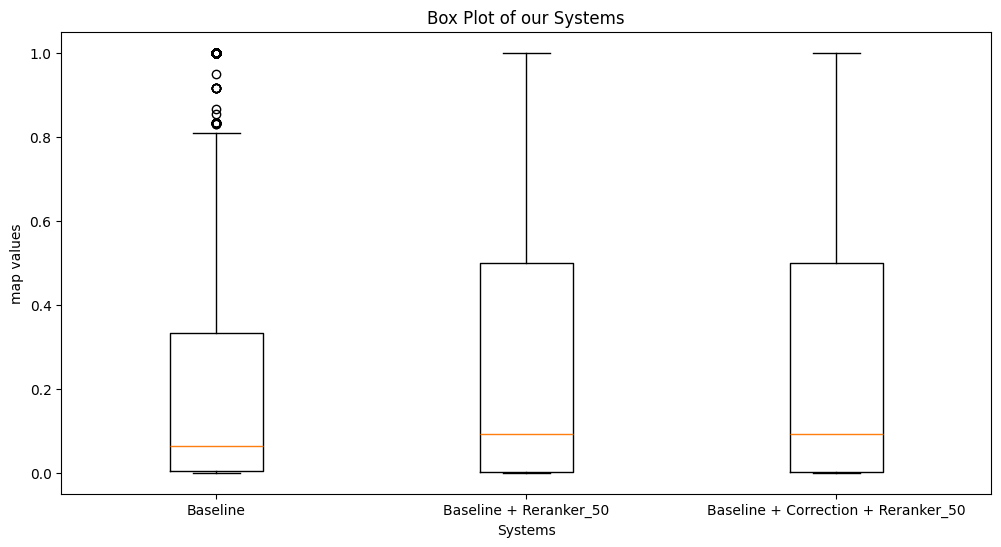
\includegraphics[height=3.5cm]{figure/box_ap_3.png} \\
2023/06 & 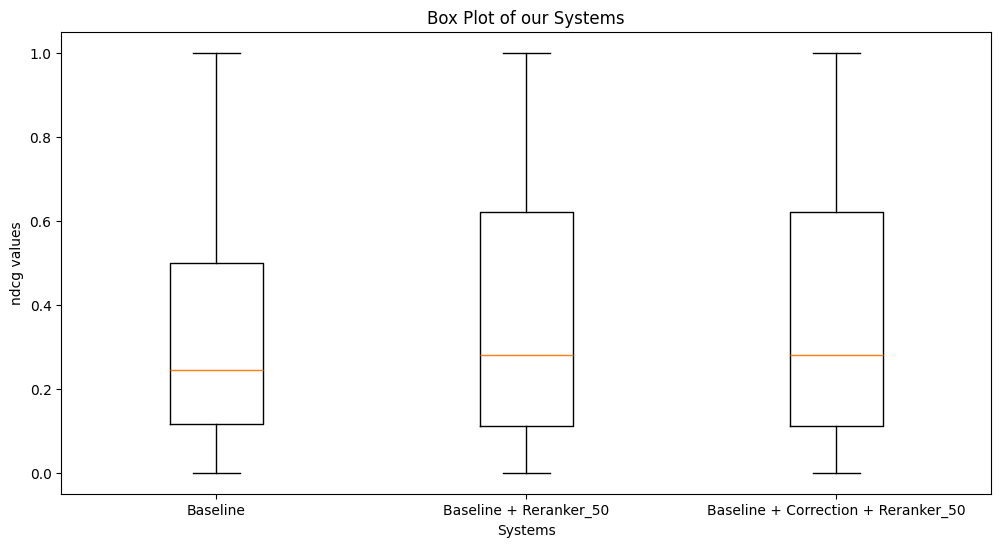
\includegraphics[height=3.5cm]{figure/box_ndcg_3.png} & 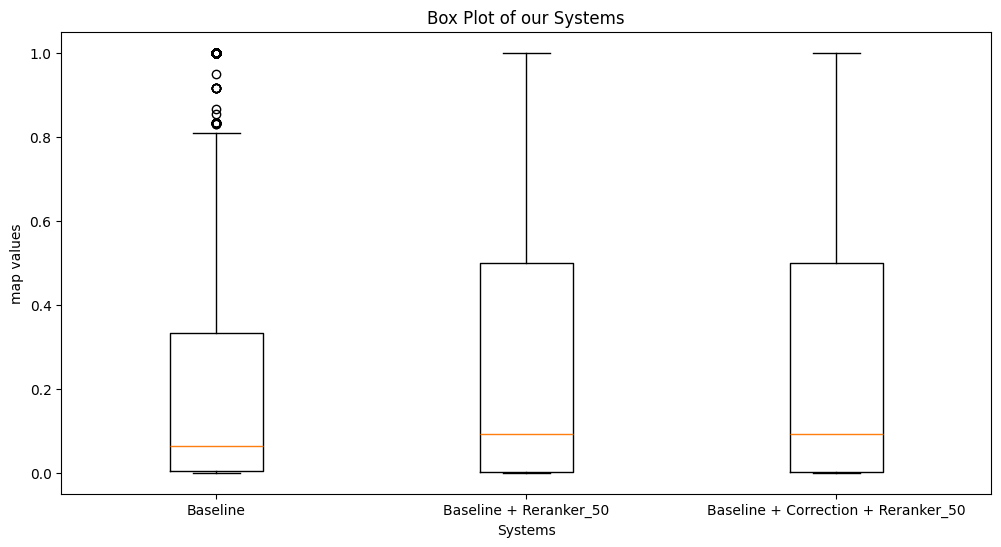
\includegraphics[height=3.5cm]{figure/box_ap_3.png} \\
2023/07 & 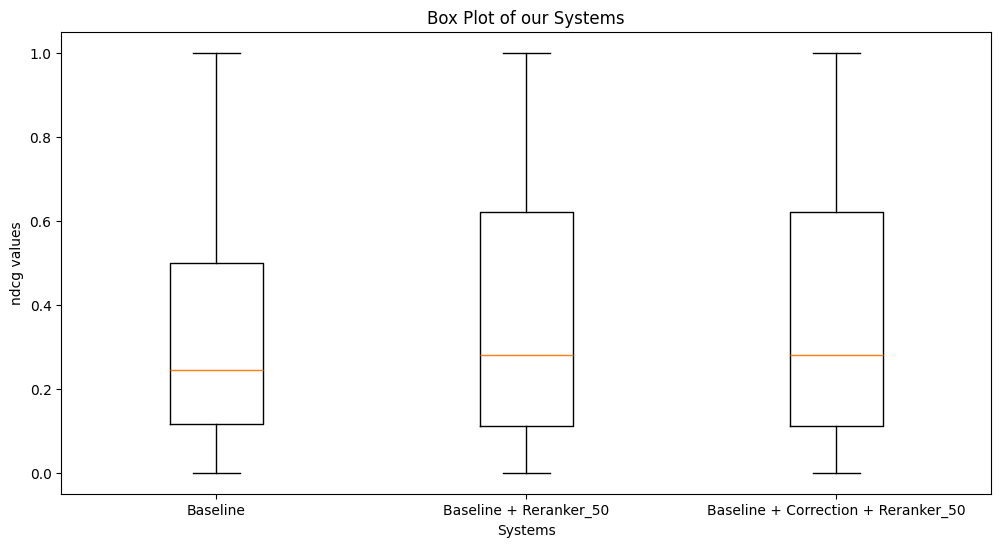
\includegraphics[height=3.5cm]{figure/box_ndcg_3.png} & 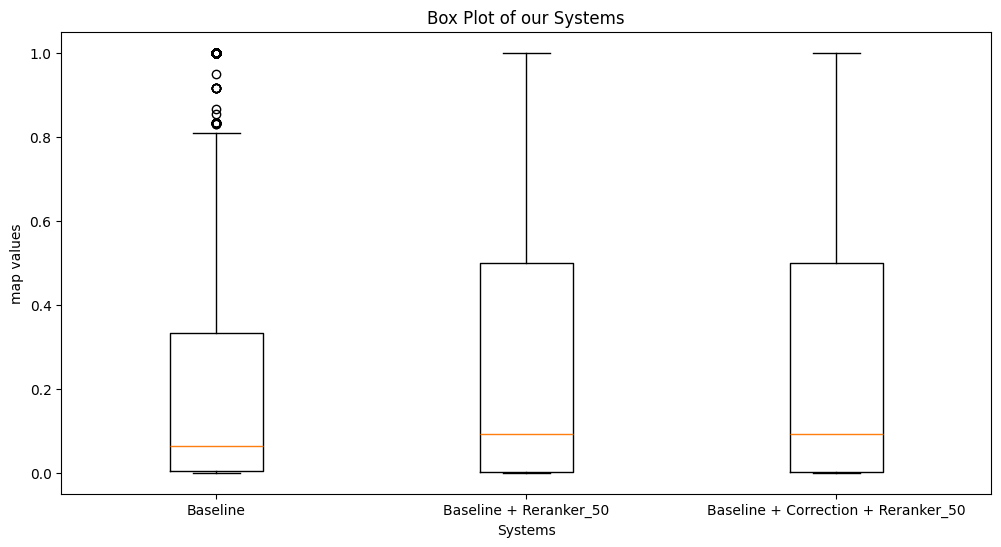
\includegraphics[height=3.5cm]{figure/box_ap_3.png} \\
2023/08 & 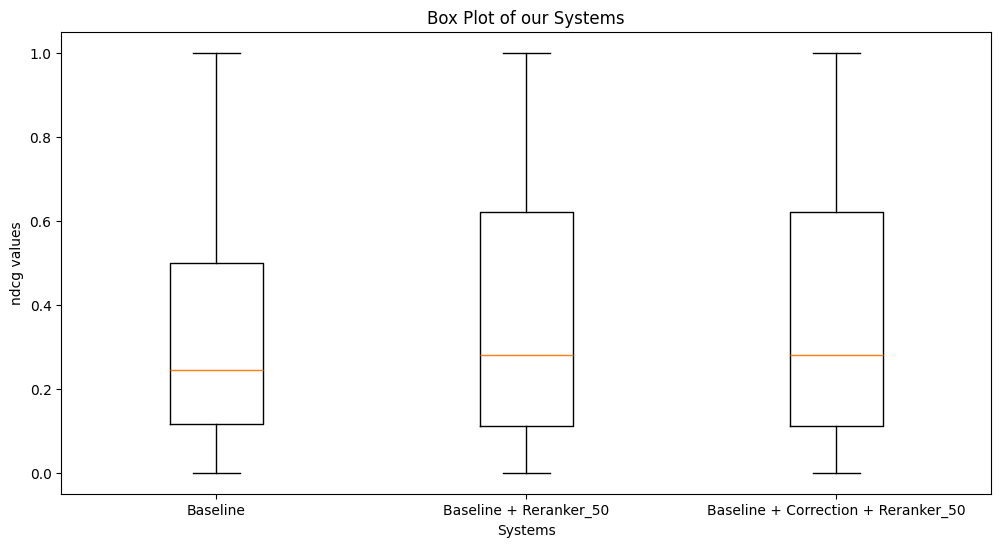
\includegraphics[height=3.5cm]{figure/box_ndcg_3.png} & 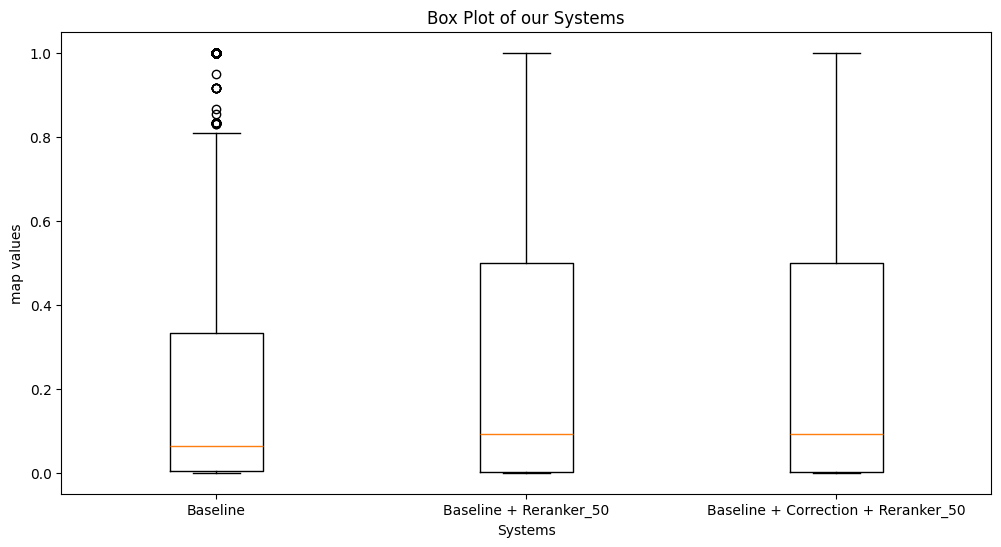
\includegraphics[height=3.5cm]{figure/box_ap_3.png} \\
\hline
\end{tabular}




The baseline system (Phrase + Fuzzy + Start + Highlights) shows consistent nDCG values ranging approximately from 0.22 to 0.27 and MAP values from 0.31 to 0.38 across the months March to August 2023.

Adding the \texttt{Reranker\_50} improves both nDCG and MAP scores noticeably in all months compared to the baseline.

The combination of \texttt{Correction + Reranker\_50} either matches or slightly improves over the \texttt{Reranker\_50} alone, except for April 2023, where values are missing (0.0).

Overall, reranking methods enhance retrieval quality significantly over the baseline.

For every month (March to August 2023), the ANOVA tests on heldout collections show:

\begin{itemize}
    \item Highly significant effects of the system ($p < 0.0001$) on both nDCG and AP, indicating that different systems (Baseline, Baseline + Reranker, Baseline + Correction + Reranker) perform differently with high confidence.
    \item Significant variance attributed to topics, confirming topic-level differences.
    \item Relatively low error variance compared to the effects, supporting reliability of the results.
\end{itemize}
